\chapter{Resultados} \label{cap:resultados}

Este capítulo exibe os resultados computacionais dos algoritmos propostos no Capítulo~\ref{cap:metodologia} para o caso do PML, para cada instância foi gerado um conjunto com 100 soluções iniciais aleatórias que foram submetidas aos métodos para comparação dos resultados.

Quando há referência à melhoria na solução (\textit{Imp}), esta melhoria pode ser calculada pelo quociente do valor da solução inicial pela solução final, ou seja:
\begin{equation}\label{eq:calculateImprovement}
Imp = \frac{f(\textrm{solução inicial})}{f(\textrm{solução final})}
\end{equation}

Desta forma quanto maior for o valor da melhoria ($Imp$) mais o método melhorou o valor da solução inicial.

\section{Instâncias} \label{sec:instancias}

Todas as instâncias usadas nos testes computacionais e cujas configurações de lançamento foram descritas na Tabela~\ref{tab:neighborhoodsLaunchConfigurarion} são as mesmas usadas em~\cite{wamca2016}.
Para o RVND foi feita uma implementação do algoritmo clássico (Algoritmo~\ref{alg:rvnd}) e também a implementação dataflow mencionada na Figura~\ref{fig:rvndGraph} fazendo uso de uma máquina.
Para o caso do DVND foi utilizada a implementação clássica (Algoritmo~\ref{alg:dvnd}) e a implementação dataflow proposta (Figura~\ref{fig:dvndGraph}), os resultados foram obtidos com diferentes números de máquinas e os mesmos são indicados conforme o caso.

\section{Implementação e ambiente computacional}\label{sec:amb}

A implementação para cada algoritmo proposto no Capítulo~\ref{cap:metodologia} utiliza a linguagem de programação \textit{C++11} em conjunto com a API CUDA\texttrademark, para a implementação dos grafos e do ambiente dataflow foi utilizada a biblioteca Sucuri~\cite{sucuri-original}\footnote{Disponível em \url{https://github.com/tiagoaoa/Sucuri}} implementada em Python, para a integração entre o dataflow e o código CUDA foi utilizada a biblioteca SimplePyCuda~\cite{simple-pycuda}\footnote{Disponível em \url{https://github.com/igormcoelho/simple-pycuda}}. As implementações com múltiplas threads usaram a biblioteca OpenMP.
%As implementações foram compiladas através do \textit{GCC} \textit{(GNU Compiler Collection)}\footnote{O GCC está disponível no seguinte sítio eletrônico: \url{https://gcc.gnu.org/}.} com a \textit{flag} de otimização $-O3$.
O ambiente computacional utilizado em todos os testes neste trabalho consiste de 4 máquinas com a seguinte configuração:

\begin{itemize}
    \item Processador Intel\textregistered Core\texttrademark i7-4820K 3.7 GHz (4 núcleos);
    \item 8 GB de memória RAM;
    \item Sistema Operacional Ubuntu 14.10 (x64);
    \item NVIDIA GeForce GTX 780 com 2304 CUDA cores.
\end{itemize}

\newcommand{\figureDvndOrRvndDcDd}[7]{
% #1 {box, scatter}, #2 {count, imp, time}, #3 {instance number}, #4 {Tempo, Melhoria}, #5 tamanho instância, #6 {DVND, RVND}, #7 {dvnd, rvnd}
\begin{figure}%
    \centering
    \includegraphics[scale=0.9]{figuras/#7/dc_dd/#1/#7_#1100sol_#2_in#3.png}
    \caption{#4 do #6 para a instância #3 de tamanho #5. $m$ indica o número de máquinas, \textit{DC} refere-se ao #6 clássico e \textit{DD} ao #6 implementado em dataflow.}%
    \label{fig:#2_#7DcDd_in#3}%
\end{figure}
}

\newcommand{\figureDvndDcDd}[5]{
% #1 {box, scatter}, #2 {count, imp, time}, #3 {instance number}, #4 {Tempo, Melhoria}, #5 tamanho instância
    \figureDvndOrRvndDcDd{#1}{#2}{#3}{#4}{#5}{DVND}{dvnd}
}

\newcommand{\figureRvndDcDd}[5]{
% #1 {box, scatter}, #2 {count, imp, time}, #3 {instance number}, #4 {Tempo, Melhoria}, #5 tamanho instância
    \figureDvndOrRvndDcDd{#1}{#2}{#3}{#4}{#5}{RVND}{rvnd}
}

\newcommand{\tabelaEstatisticasGeral}[6]{
% #1 Descrição, #2 label, #3 {dvnd, rvnd}, #4 {DVND, RVND}, #6 DD/DC, #6 Conteúdo
\begin{table}[ht]
    \centering
    \begin{tabular}{c|ccc|cc|ccc|cc|c}
        \hline \hline
        \# & Tipo & $m$ & $n$ & $min$ & $max$ & 1Q & 2Q & 3Q & $\overline{x}$ & $\sigma$ & $p-valor$ \\ \hline
        #6
    \end{tabular}
    \caption{#1 #4 #5
        Instância (\#), tipo de implementação (Tipo), número de máquinas ($m$), tamanho da instância ($n$), valor mínimo ($min$), máximo ($max$), primeiro quartil (1Q), mediana (2Q), terceiro quartil (3Q), média ($\overline{x}$), desvio padrão ($\sigma$) e p-valor para o teste de Wilcox entre as versões (valores em negrito quando $p-valor > 0.05$).
    }
    \label{tab:#3DcDd#2}
\end{table}
}

\newcommand{\tabelaEstatisticas}[5]{
    \tabelaEstatisticasGeral{#1}{#2}{#3}{#4}{na implementação clássica (DC) e a proposta de implementação usando dataflow (DD).}{#5}
}

\newcommand{\figureDvndSogMog}[7]{
% #1 {box, scatter}, #2 {count, imp, time}, #3 {instance number}, #4 {Tempo, Melhoria}, #5 tamanho instância, #6 {DVND, RVND}, #7 {dvnd, rvnd}
\begin{figure}%
    \centering
    \includegraphics[scale=0.9]{figuras/#7/sog_mog/#1/#7_#1100sol_#2_in#3.png}
    \caption{#4 do #6 para a instância #3 de tamanho #5. \textit{SOG} refere-se a uma porta de saída e \textit{MOG} a múltiplas portas de saída.}%
    \label{fig:#2_#7SogMog_in#3}%
\end{figure}
}

\newcommand{\figureDvndGdvnd}[9]{
% #1 {box, scatter}, #2 {count, imp, time}, #3 {instance number}, #4 {Tempo, Melhoria}, #5 tamanho instância, #6 {DVND, RVND}, #7 {dvnd, rvnd}, #8 {man_time, full_time}, #9 {man, dvnd} #10 descricao
\begin{figure}%
    \centering
    \includegraphics[scale=0.9]{figuras/#7/#8/#1/#9_#1100sol_#2_in#3.png}
    \caption{#4 do #6 para a instância #3 de tamanho #5. \textit{DVND} refere-se ao tempo gasto pelo algoritmo de mesmo nome, para \textit{GDVND} é análogo ao anterior, no caso do \textit{GDVND-MAN} este se refere ao tempo do GDVND subtraido do tempo para gerenciar os movimentos.}%
    \label{fig:#2_#7_#8_in#3}%
\end{figure}
}

\newcommand{\figureDvndGdvndTime}[8]{
    \figureDvndGdvnd{#1}{#2}{#3}{#4}{#5}{#6}{#7}{man_time}{man}
}

\newcommand{\figureGdvndDvndRvnd}[9]{
% #1 {box, scatter}, #2 {count, imp, time}, #3 {instance number}, #4 {Tempo, Melhoria}, #5 tamanho instância, #6 {DVND, RVND}, #7 {dvnd, rvnd}, #8 {man_time, full_time}, #9 {man, dvnd} #10 descricao
\begin{figure}%
    \centering
    \includegraphics[scale=0.9]{figuras/#7/#8/#1/#9_#1100sol_#2_in#3.png}
    \caption{#4 do #6 para a instância #3 de tamanho #5. \textit{DVND}, \textit{GDVND} e \textit{RVND} referem-se ao tempo gasto pelos algoritmos de mesmo nome.}%
    \label{fig:#2_#7_#8_in#3}%
\end{figure}
}

% \subfloat[$m=#1$]{{ %scale=0.225
%         \includegraphics[scale=0.425]{figuras/dvnd/n#1/time#2.png}
%         \label{fig:timeDvndRvnd_n#1in#2}
%     }}%
% #1 {dvnd, rvnd, gdvnd}, #2 {sog_mog, dc_dd}, #3 {time, imp}, #4 in, #5 tamanho, #6 {box, scatter}
\newcommand{\subFig}[6]{
    \subfloat[][Instância #4, $n=#5$]{
        \includegraphics[width=.5\linewidth]{figuras/#1/#2/#6/#1_#6100sol_#3_in#4.png}
		\label{fig:#1_#2_#3_in#4}
    }
% 	\begin{subfigure}{0.45\textwidth} % dvnd_box100sol_imp_in0
% 		\includegraphics[scale=0.425]{figuras/#1/#2/#6/#1_#6100sol_#3_in#4.png}
% 		\caption{Instância #4, $n=#5$}
        % \label{fig:#1_#2_#3_in#4}
    % \end{subfigure}
}

\newcommand{\subFigBox}[5]{
	\subFig{#1}{#2}{#3}{#4}{#5}{box}
}

\newcommand{\subFigScatter}[5]{
	\subFig{#1}{#2}{#3}{#4}{#5}{scatter}
}

% #1 {dvnd, rvnd, gdvnd}, #2 {sog_mog, dc_dd}, #3 {time, imp}, #4 {box, scatter}, #5 {Tempo do DVND...}
\newcommand{\multiFigureInstanciasGeral}[5]{
	\begin{figure}[ht]
		\centering
		\subFig{#1}{#2}{#3}{0}{52}{#4}
		~
		\subFig{#1}{#2}{#3}{1}{100}{#4}
		
		\subFig{#1}{#2}{#3}{2}{226}{#4}
		~
		\subFig{#1}{#2}{#3}{3}{318}{#4}

        \includegraphics[width=.9\linewidth]{figuras/#1/#2/#4/#1_#4100sol_#3_legenda.png}
		\caption{#5 Instâncias 0 a 3.}
		\label{fig:#1_#2_#3_in0_4}
	\end{figure}
	
	\begin{figure}[ht]
		\centering
		\subFig{#1}{#2}{#3}{4}{501}{#4}
		~
		\subFig{#1}{#2}{#3}{5}{657}{#4}
		
		\subFig{#1}{#2}{#3}{6}{783}{#4}
		~
		\subFig{#1}{#2}{#3}{7}{1001}{#4}

		\includegraphics[width=.9\linewidth]{figuras/#1/#2/#4/#1_#4100sol_#3_legenda.png}
		\caption{#5 Instâncias 4 a 7.}
		\label{fig:#1_#2_#3_in5_7}
	\end{figure}
}

% #1 {dvnd, rvnd, gdvnd}, #2 {sog_mog, dc_dd}, #3 {time, imp}, #4 {Tempo do DVND...}
\newcommand{\multiFigureInstancias}[4]{
    \multiFigureInstanciasGeral{#1}{#2}{#3}{box}{#4}
}


\section{Dataflow} \label{sec:conceitosDataflow}
% Essa parte tá bem próxima da tese do Marzulo

Atualmente os processadores no mercado de computadores seguem, em geral, o modelo de \textit{Von Neumann}.
No referido modelo, a execução das instruções é guiada por um fluxo de controle, ou seja, segundo a ordem que aparecem no programa, desta forma se faz necessário um \textit{Program Counter} (Contador de Programa) para indicar qual a próxima instrução a ser executada.
O contador também pode ser alterado por instruções de desvio, e laços de repetição ou qualquer tipo de comando de execução condicional.

Note que este modelo é intrinsecamente sequencial. No entanto, tenta-se resgatar paralelismo em nível de instruções com técnicas como pipelining~\cite{patterson2003computerOrganization}, predição de desvio~\cite{patterson2003computerOrganization} e renomeamento de registradores~\cite{patterson2012}.

O modelo dataflow~\cite{2468, Swanson2003, 642111, Davis:1978:ASM:800094.803050, 714523, Shimada:1986:EPD:17356.17383, Kishi:1983:DDD:1067651.801661, Grafe:1989:EDP:74925.74930, 134511, Swanson:2007:WA:1233307.1233308} expõe paralelismo de forma natural.
Neste modelo, as instruções são executadas de acordo com o fluxo de dados, ou seja, assim que todos os seus operandos de entrada estiverem disponíveis.

No modelo dataflow os programas são escritos como um grafo de fluxo de dados onde os nós representam as instruções e as arestas direcionadas indicam as dependências de dados.
Assim $A \rightarrow B$ indica que $A$ produz um dado que é enviado como entrada para $B$ após ter sido processado.
Cabe lembrar que este modelo é adotado nas máquinas de Von Neumann para extrair paralelismo ao implementar o mecanismo de execução fora-de-ordem com escalonamento dinâmico baseado em fluxo de dados~\cite{tomasulo}, contudo limitado o paralelismo pela emissão das instruções que permanece seguindo o fluxo de controle.
Numa arquitetura que segue totalmente o fluxo de dados as instruções não são emitidas segundo se apresentam no programa, instruções distintas podem executar concorrentemente.

Na Figura~\ref{fig:dataflowExemploPython} pode ser visto um programa simples, à esquerda é mostrado o código e à direita sua tradução no grafo de fluxo de dados associado, note que as instruções de soma e multiplicação podem ser executadas em paralelo ou qualquer ordem sem alterar o resultado final.

\begin{figure}
    \centering
    \begin{minipage}{.3\textwidth}
        \centering
\begin{minted}{python}
a = 10
b = 9
c = 3
d = 8
e = a * b
f = c + d
if e > f:
  g = (a - b) * a
else:
  g = (c - d) * d
\end{minted}
    \end{minipage}
    \begin{minipage}{.675\textwidth}
        \centering %width=.655\linewidth
        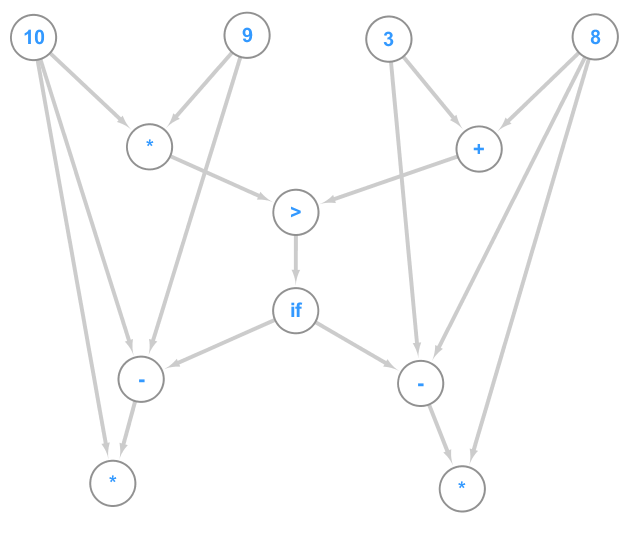
\includegraphics[scale=.7]{figuras/dataflow/pythonCodeDf.png}
    \end{minipage}
    \caption{Exemplo de conversão código para grafo de dependências.
    À esquerda pode ser visto um trecho de código em \emph{python} ao passo que à direita é exibido o grafo dataflow associado.}
    \label{fig:dataflowExemploPython}
\end{figure}

% \subsection{Sucuri} \label{sect:sucuri}

Sucuri \cite{sucuri-original} is a minimalistic Dataflow library for Python language that allows programmers to naturally exploit parallelism through dataflow execution on Von Neumann machines. Sucuri allows transparent execution on computer cluster, relying on Python mechanisms for object serialization (\emph{Pickle}).

Conceptually, a dataflow graph is comprised of nodes that represent tasks, which can be fine-grained (as instructions) or coarse-grained (as functions). Edges connecting nodes represent data-dependencies, meaning a source node will produce a result that will be used by the destination node. When a certain node receives all necessary inputs though its incident edges, it can be dispatched to execution.

Figure \ref{fig:arch} shows Sucuri's structure, where it is possible to observe three main components: \texttt{Graph}, \texttt{Scheduler} and \texttt{Worker}. 

The \texttt{Graph} is just a container object for nodes that represent a dataflow application, each containing:
\begin{itemize}
    \item The list of inputs received so far. When all necessary operands are receive a \emph{matching} occurs and node execution will be triggered.
    \item The function (computation) that should be executed when matching happens for that node.
    \item A list of destination nodes that should receive the result produced.
    \item Specific attributes, such as an unique id that can be used for assigning work to a set of nodes (like in a fork-join approach).
\end{itemize}

When used in a cluster of computers, each of the aforementioned components is replicated in each machine of the cluster, except for the Scheduler, meaning Sucuri adopts a centralized pool of tasks. In \cite{sucuri-distribuida} Sucuri authors implement and evaluate a distributed scheduler for Sucuri, but this version is not employed in this work.

\begin{figure}[htbp]
    \centering
    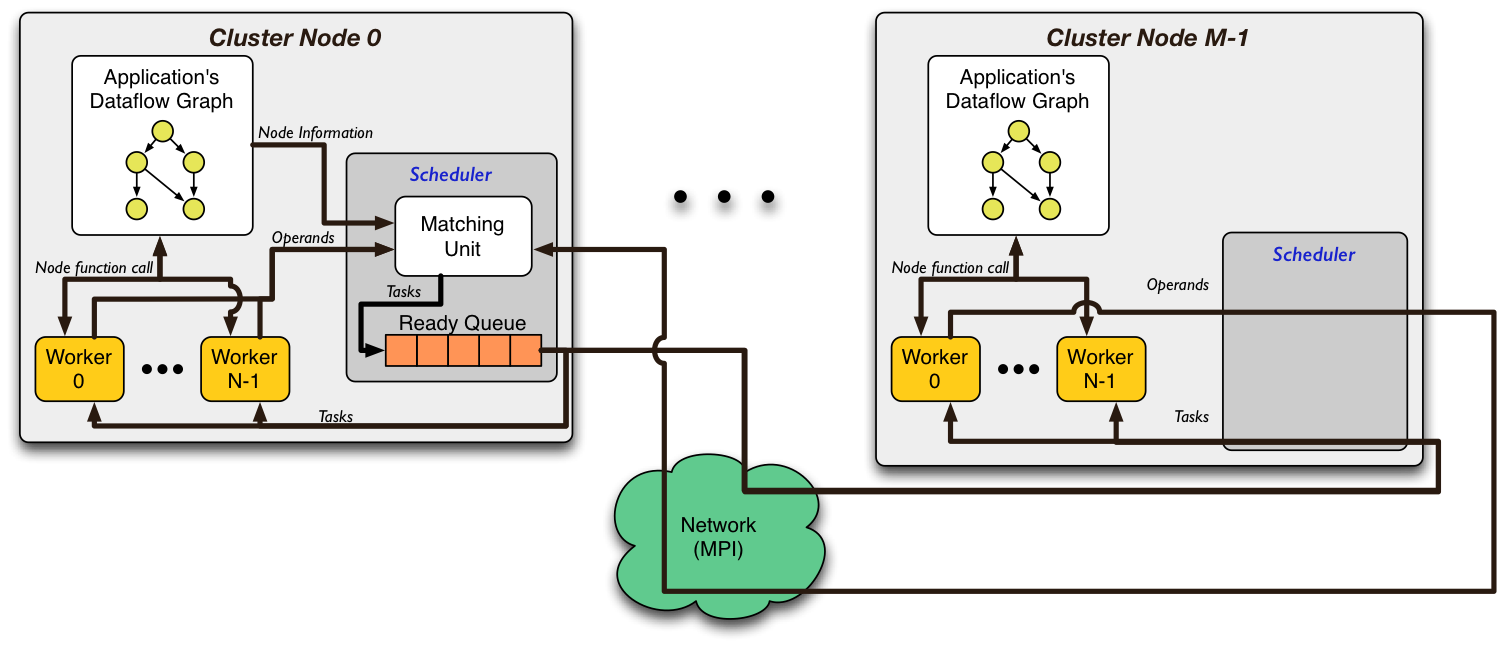
\includegraphics[scale=0.65]{figuras/dataflow/SucuriArchitectureHorizonal.png}
    \caption{The Sucuri Architecture (from \cite{sucuri-original}). The same structure is replicated in each node but only the Scheduler from Cluster Node 0 contains the Matching Unit and the Ready Queue. It is responsible for receiving operands from local Workers and from the others Schedulers and also to generate tasks and put them into the Ready Queue.}
    \label{fig:arch}
\end{figure}

The main \texttt{Scheduler}, placed at Cluster Node 0, is composed of a Matching Unit, a Ready Queue and a Waiting Queue. It is responsible for delivering all operands to the operand list of its destination Node in the Graph. If a match happens, a task is created and put in the Ready Queue. When workers are idle they will request tasks to the \texttt{Scheduler}, that would be fetched from the Ready Queue. The \texttt{Scheduler} placed in the other cluster nodes are more simple and only forwards tasks from the main \texttt{Scheduler} to their local workers and operands from their workers to the main \texttt{Scheduler}. The graph is replicated in all nodes of the Cluster but only the graph in node 0 can receive operands from the main \texttt{Scheduler}.

All communication intra-node between the main components cited above is done via shared memory and between Schedulers from different nodes is done via interface.

Each node of a Sucuri graph is associated with a function that can be implemented by programmers and pass them to node instantiation when creating the dataflow graph. After instantiating the nodes, the programmer can then proceed to connect them using the \texttt{add\_edge()} method, which basically creates a new dependency in the dataflow graph. When the scheduler dispatches a task for execution in a certain worker, that worker will call the \texttt{run()} method of the node corresponding to that task. In most cases, this \texttt{run()} method will just act as a wrapper that calls the function associated with the node during the construction of the graph and send the values returned by the function call to the main scheduler.

Sucuri also provides a set of special nodes that could help programmers devise applications that follow some parallel patterns. For example, a software pipeline application for Sucuri is presented in Fig.~\ref{fig:pipeline}. Panel $A$ shows a graph representation of this pattern and panel $B$ the Sucuri's code for this operation. Notice how new nodes are creates (lines 11-13), added to the graph (lines 17-19) and how edges connecting the nodes are defined (lines 21 and 22). Also, notice the instantiation of the scheduler (line 6) and how to start the schedule after the dataflow graph is defined (line 23).

Figure \ref{fig:pipeline} also shows how a special node \texttt{Source} receives an \emph{iterable} Python object (for instance, a list or a file descriptor) at instantiation. During program execution, the \texttt{run()} method of the \emph{Source} node will be fired only once, since this node works as a root, i.e., has no input operands from the graph and serves to initiate the computation. The execution of such method, however, will typically last until the contents of the iterable object are exhausted. By default the \texttt{Source} node will loop over the iterable object and produce several outputs (messages) that would trigger the execution of the pipeline multiple times. 

Notice that the last node of the pipeline is a special \texttt{Serializer} node, that is responsible for writing the data to a file. It is possible for the data produced by the \texttt{Source} node to be processed out of order by the second node, since the multiple tasks may be scheduled to different workers. Therefore, it is necessary to reorder the data before writing it to the file, in the \texttt{Serializer} node. For that purpose, the data produced by the \texttt{Source} node must be encapsulated in a \texttt{TaggedValue} object, which contains a \texttt{tag} attribute, indicating its position in the ordered data set. The middle node will also send the filtered data inside of a \texttt{TaggedValue} object, with the same tag of the chunk of data it received. The \texttt{Serializer} node then, upon receiving data from the filter node, will store it in a buffer sorted according to the tag. If the tag of the last piece of data received corresponds to the next data to be written to the file, the \texttt{Serializer} node proceeds to pop data from the sorted buffer and write to the file until there is a gap in the ordering, i.e. the chunk of data that is the next to be written has not arrived yet. If the data received by the \texttt{Serializer} is out of order, the node just stores it in the sorted buffer and waits for more data. The \texttt{pin\(\)} method is used to pin the node to a certain worker, which will make it only be executed by that worker. In the case of the example, we pin the nodes that performs I\/O operations on disk to the workers that have direct access to that disk. 

\begin{figure}[htbp]
    \centering
    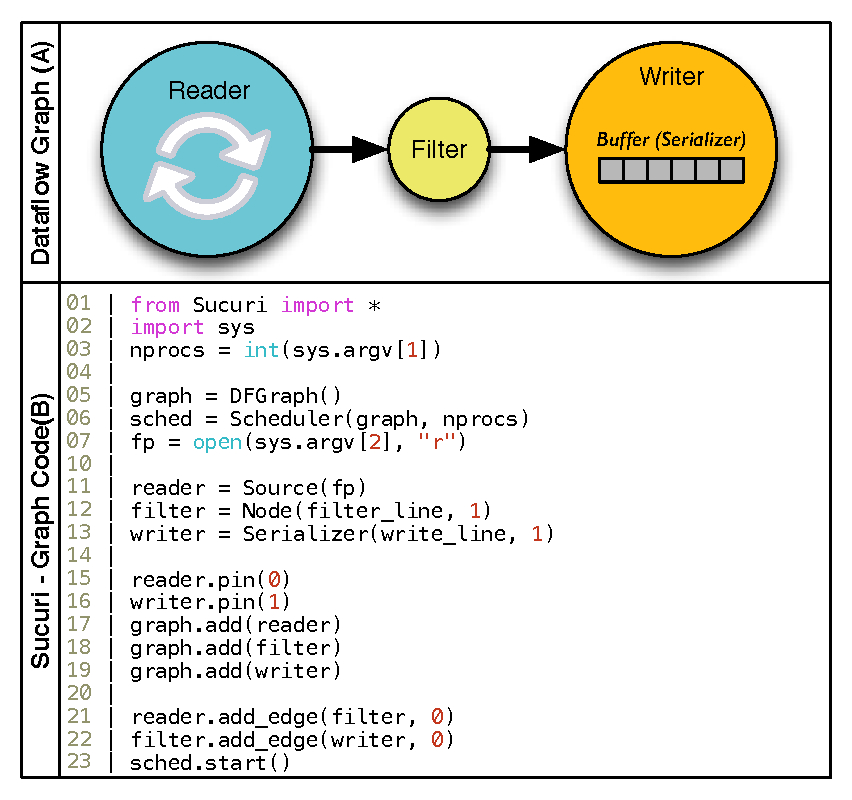
\includegraphics[scale=0.75]{figuras/dataflow/pipeline.eps} 
    \caption{Pipelining with Sucuri. 
    %The data is read from the disk by \texttt{Reader} node encapsulated in a \texttt{TaggedValue} object while a filter is applied by \texttt{Filer} node in a data read previously. As the \texttt{Filter} finish, the \texttt{Writer} node receives and store them in buffer sorted according to the tag. If the tag of the last piece of data received corresponds to the next data to be written to the file, the \texttt{Writer} node proceeds to pop data from the sorted buffer and write to the file.
    Panel $A$ shows the dataflow graph of the application, panel $B$ describes the graph using Sucuri.}
    \label{fig:pipeline}
\end{figure}

One interesting modeling feature that we explore in this paper consists in exploring coarse-grained programming in Sucuri together with fine-grained computing on GPU. This results in a heterogeneous Dataflow/Von Neumann computing, with dataflow nodes performing high performance GPU computing.
This strategy provides greater flexibility for the design of novel algorithms, with greater simplicity than adopting a single computing paradigm (dataflow or von Neumann).



\section{Dataflow} \label{sec:conceitosDataflow}
% Essa parte tá bem próxima da tese do Marzulo

Atualmente os processadores no mercado de computadores seguem, em geral, o modelo de \textit{Von Neumann}.
No referido modelo, a execução das instruções é guiada por um fluxo de controle, ou seja, segundo a ordem que aparecem no programa, desta forma se faz necessário um \textit{Program Counter} (Contador de Programa) para indicar qual a próxima instrução a ser executada.
O contador também pode ser alterado por instruções de desvio, e laços de repetição ou qualquer tipo de comando de execução condicional.

Note que este modelo é intrinsecamente sequencial. No entanto, tenta-se resgatar paralelismo em nível de instruções com técnicas como pipelining~\cite{patterson2003computerOrganization}, predição de desvio~\cite{patterson2003computerOrganization} e renomeamento de registradores~\cite{patterson2012}.

O modelo dataflow~\cite{2468, Swanson2003, 642111, Davis:1978:ASM:800094.803050, 714523, Shimada:1986:EPD:17356.17383, Kishi:1983:DDD:1067651.801661, Grafe:1989:EDP:74925.74930, 134511, Swanson:2007:WA:1233307.1233308} expõe paralelismo de forma natural.
Neste modelo, as instruções são executadas de acordo com o fluxo de dados, ou seja, assim que todos os seus operandos de entrada estiverem disponíveis.

No modelo dataflow os programas são escritos como um grafo de fluxo de dados onde os nós representam as instruções e as arestas direcionadas indicam as dependências de dados.
Assim $A \rightarrow B$ indica que $A$ produz um dado que é enviado como entrada para $B$ após ter sido processado.
Cabe lembrar que este modelo é adotado nas máquinas de Von Neumann para extrair paralelismo ao implementar o mecanismo de execução fora-de-ordem com escalonamento dinâmico baseado em fluxo de dados~\cite{tomasulo}, contudo limitado o paralelismo pela emissão das instruções que permanece seguindo o fluxo de controle.
Numa arquitetura que segue totalmente o fluxo de dados as instruções não são emitidas segundo se apresentam no programa, instruções distintas podem executar concorrentemente.

Na Figura~\ref{fig:dataflowExemploPython} pode ser visto um programa simples, à esquerda é mostrado o código e à direita sua tradução no grafo de fluxo de dados associado, note que as instruções de soma e multiplicação podem ser executadas em paralelo ou qualquer ordem sem alterar o resultado final.

\begin{figure}
    \centering
    \begin{minipage}{.3\textwidth}
        \centering
\begin{minted}{python}
a = 10
b = 9
c = 3
d = 8
e = a * b
f = c + d
if e > f:
  g = (a - b) * a
else:
  g = (c - d) * d
\end{minted}
    \end{minipage}
    \begin{minipage}{.675\textwidth}
        \centering %width=.655\linewidth
        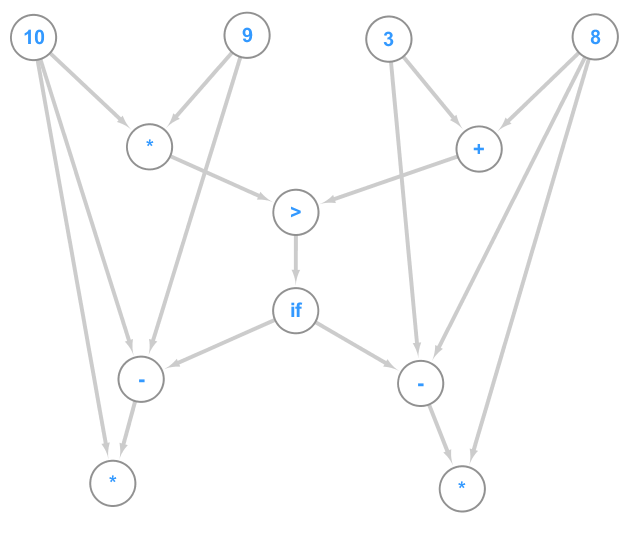
\includegraphics[scale=.7]{figuras/dataflow/pythonCodeDf.png}
    \end{minipage}
    \caption{Exemplo de conversão código para grafo de dependências.
    À esquerda pode ser visto um trecho de código em \emph{python} ao passo que à direita é exibido o grafo dataflow associado.}
    \label{fig:dataflowExemploPython}
\end{figure}

% \subsection{Sucuri} \label{sect:sucuri}

Sucuri \cite{sucuri-original} is a minimalistic Dataflow library for Python language that allows programmers to naturally exploit parallelism through dataflow execution on Von Neumann machines. Sucuri allows transparent execution on computer cluster, relying on Python mechanisms for object serialization (\emph{Pickle}).

Conceptually, a dataflow graph is comprised of nodes that represent tasks, which can be fine-grained (as instructions) or coarse-grained (as functions). Edges connecting nodes represent data-dependencies, meaning a source node will produce a result that will be used by the destination node. When a certain node receives all necessary inputs though its incident edges, it can be dispatched to execution.

Figure \ref{fig:arch} shows Sucuri's structure, where it is possible to observe three main components: \texttt{Graph}, \texttt{Scheduler} and \texttt{Worker}. 

The \texttt{Graph} is just a container object for nodes that represent a dataflow application, each containing:
\begin{itemize}
    \item The list of inputs received so far. When all necessary operands are receive a \emph{matching} occurs and node execution will be triggered.
    \item The function (computation) that should be executed when matching happens for that node.
    \item A list of destination nodes that should receive the result produced.
    \item Specific attributes, such as an unique id that can be used for assigning work to a set of nodes (like in a fork-join approach).
\end{itemize}

When used in a cluster of computers, each of the aforementioned components is replicated in each machine of the cluster, except for the Scheduler, meaning Sucuri adopts a centralized pool of tasks. In \cite{sucuri-distribuida} Sucuri authors implement and evaluate a distributed scheduler for Sucuri, but this version is not employed in this work.

\begin{figure}[htbp]
    \centering
    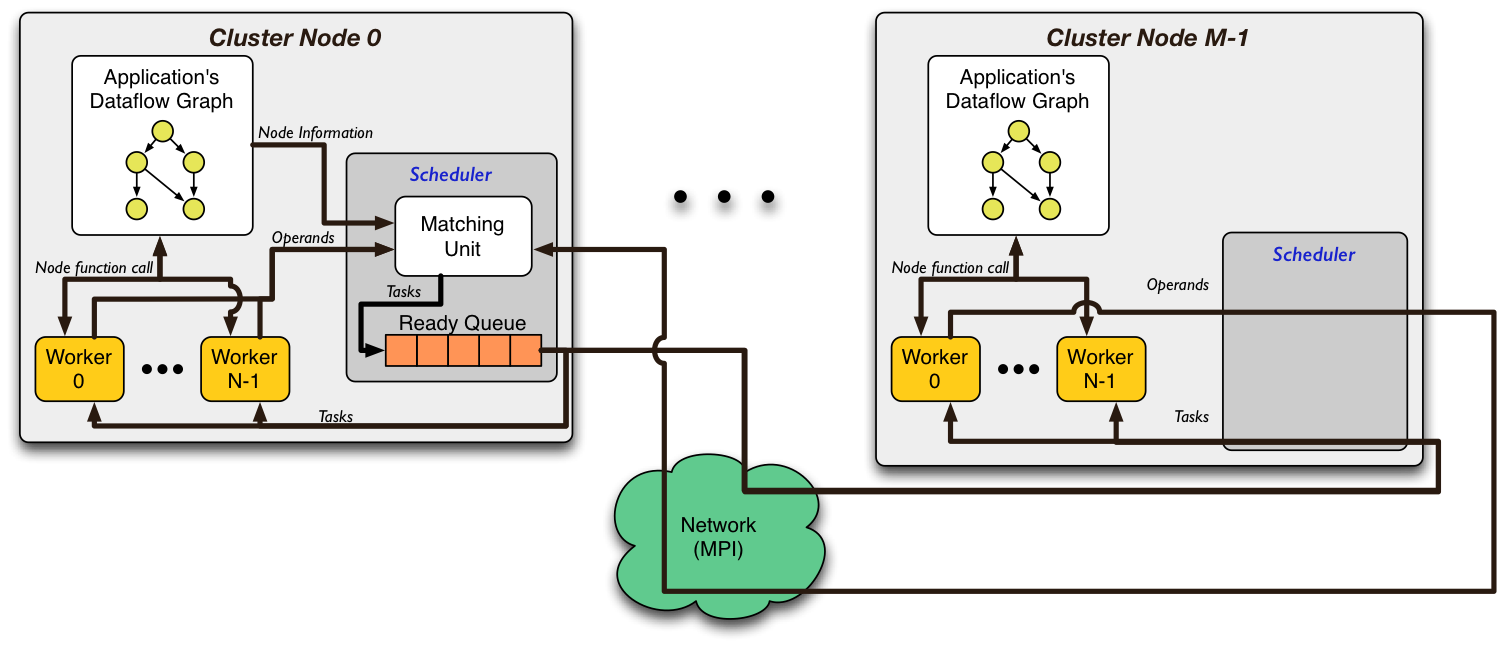
\includegraphics[scale=0.65]{figuras/dataflow/SucuriArchitectureHorizonal.png}
    \caption{The Sucuri Architecture (from \cite{sucuri-original}). The same structure is replicated in each node but only the Scheduler from Cluster Node 0 contains the Matching Unit and the Ready Queue. It is responsible for receiving operands from local Workers and from the others Schedulers and also to generate tasks and put them into the Ready Queue.}
    \label{fig:arch}
\end{figure}

The main \texttt{Scheduler}, placed at Cluster Node 0, is composed of a Matching Unit, a Ready Queue and a Waiting Queue. It is responsible for delivering all operands to the operand list of its destination Node in the Graph. If a match happens, a task is created and put in the Ready Queue. When workers are idle they will request tasks to the \texttt{Scheduler}, that would be fetched from the Ready Queue. The \texttt{Scheduler} placed in the other cluster nodes are more simple and only forwards tasks from the main \texttt{Scheduler} to their local workers and operands from their workers to the main \texttt{Scheduler}. The graph is replicated in all nodes of the Cluster but only the graph in node 0 can receive operands from the main \texttt{Scheduler}.

All communication intra-node between the main components cited above is done via shared memory and between Schedulers from different nodes is done via interface.

Each node of a Sucuri graph is associated with a function that can be implemented by programmers and pass them to node instantiation when creating the dataflow graph. After instantiating the nodes, the programmer can then proceed to connect them using the \texttt{add\_edge()} method, which basically creates a new dependency in the dataflow graph. When the scheduler dispatches a task for execution in a certain worker, that worker will call the \texttt{run()} method of the node corresponding to that task. In most cases, this \texttt{run()} method will just act as a wrapper that calls the function associated with the node during the construction of the graph and send the values returned by the function call to the main scheduler.

Sucuri also provides a set of special nodes that could help programmers devise applications that follow some parallel patterns. For example, a software pipeline application for Sucuri is presented in Fig.~\ref{fig:pipeline}. Panel $A$ shows a graph representation of this pattern and panel $B$ the Sucuri's code for this operation. Notice how new nodes are creates (lines 11-13), added to the graph (lines 17-19) and how edges connecting the nodes are defined (lines 21 and 22). Also, notice the instantiation of the scheduler (line 6) and how to start the schedule after the dataflow graph is defined (line 23).

Figure \ref{fig:pipeline} also shows how a special node \texttt{Source} receives an \emph{iterable} Python object (for instance, a list or a file descriptor) at instantiation. During program execution, the \texttt{run()} method of the \emph{Source} node will be fired only once, since this node works as a root, i.e., has no input operands from the graph and serves to initiate the computation. The execution of such method, however, will typically last until the contents of the iterable object are exhausted. By default the \texttt{Source} node will loop over the iterable object and produce several outputs (messages) that would trigger the execution of the pipeline multiple times. 

Notice that the last node of the pipeline is a special \texttt{Serializer} node, that is responsible for writing the data to a file. It is possible for the data produced by the \texttt{Source} node to be processed out of order by the second node, since the multiple tasks may be scheduled to different workers. Therefore, it is necessary to reorder the data before writing it to the file, in the \texttt{Serializer} node. For that purpose, the data produced by the \texttt{Source} node must be encapsulated in a \texttt{TaggedValue} object, which contains a \texttt{tag} attribute, indicating its position in the ordered data set. The middle node will also send the filtered data inside of a \texttt{TaggedValue} object, with the same tag of the chunk of data it received. The \texttt{Serializer} node then, upon receiving data from the filter node, will store it in a buffer sorted according to the tag. If the tag of the last piece of data received corresponds to the next data to be written to the file, the \texttt{Serializer} node proceeds to pop data from the sorted buffer and write to the file until there is a gap in the ordering, i.e. the chunk of data that is the next to be written has not arrived yet. If the data received by the \texttt{Serializer} is out of order, the node just stores it in the sorted buffer and waits for more data. The \texttt{pin\(\)} method is used to pin the node to a certain worker, which will make it only be executed by that worker. In the case of the example, we pin the nodes that performs I\/O operations on disk to the workers that have direct access to that disk. 

\begin{figure}[htbp]
    \centering
    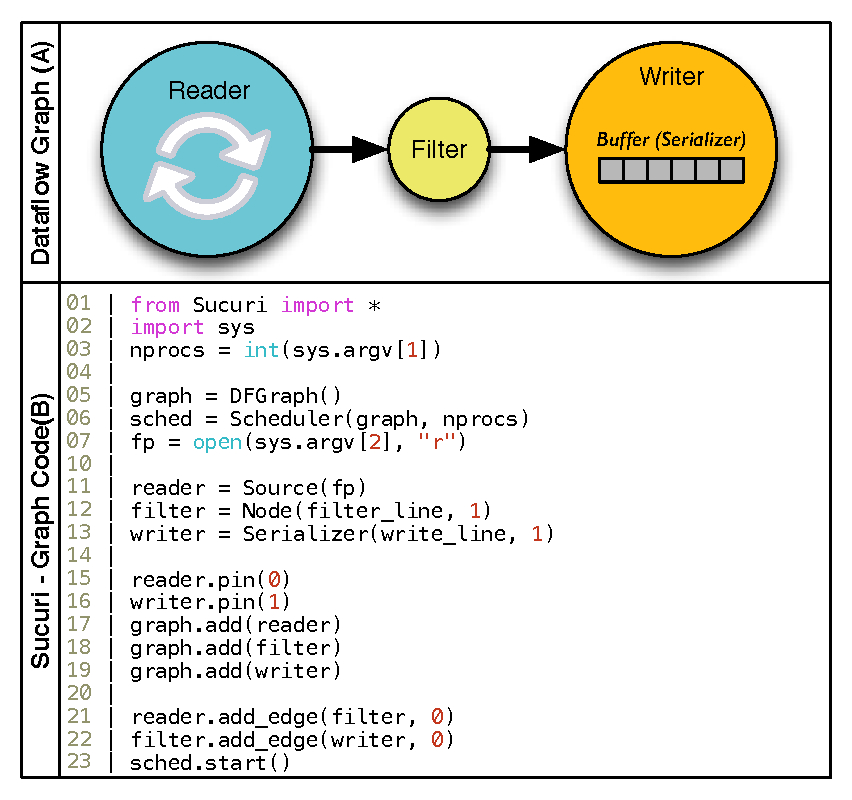
\includegraphics[scale=0.75]{figuras/dataflow/pipeline.eps} 
    \caption{Pipelining with Sucuri. 
    %The data is read from the disk by \texttt{Reader} node encapsulated in a \texttt{TaggedValue} object while a filter is applied by \texttt{Filer} node in a data read previously. As the \texttt{Filter} finish, the \texttt{Writer} node receives and store them in buffer sorted according to the tag. If the tag of the last piece of data received corresponds to the next data to be written to the file, the \texttt{Writer} node proceeds to pop data from the sorted buffer and write to the file.
    Panel $A$ shows the dataflow graph of the application, panel $B$ describes the graph using Sucuri.}
    \label{fig:pipeline}
\end{figure}

One interesting modeling feature that we explore in this paper consists in exploring coarse-grained programming in Sucuri together with fine-grained computing on GPU. This results in a heterogeneous Dataflow/Von Neumann computing, with dataflow nodes performing high performance GPU computing.
This strategy provides greater flexibility for the design of novel algorithms, with greater simplicity than adopting a single computing paradigm (dataflow or von Neumann).



\section{Dataflow} \label{sec:conceitosDataflow}
% Essa parte tá bem próxima da tese do Marzulo

Atualmente os processadores no mercado de computadores seguem, em geral, o modelo de \textit{Von Neumann}.
No referido modelo, a execução das instruções é guiada por um fluxo de controle, ou seja, segundo a ordem que aparecem no programa, desta forma se faz necessário um \textit{Program Counter} (Contador de Programa) para indicar qual a próxima instrução a ser executada.
O contador também pode ser alterado por instruções de desvio, e laços de repetição ou qualquer tipo de comando de execução condicional.

Note que este modelo é intrinsecamente sequencial. No entanto, tenta-se resgatar paralelismo em nível de instruções com técnicas como pipelining~\cite{patterson2003computerOrganization}, predição de desvio~\cite{patterson2003computerOrganization} e renomeamento de registradores~\cite{patterson2012}.

O modelo dataflow~\cite{2468, Swanson2003, 642111, Davis:1978:ASM:800094.803050, 714523, Shimada:1986:EPD:17356.17383, Kishi:1983:DDD:1067651.801661, Grafe:1989:EDP:74925.74930, 134511, Swanson:2007:WA:1233307.1233308} expõe paralelismo de forma natural.
Neste modelo, as instruções são executadas de acordo com o fluxo de dados, ou seja, assim que todos os seus operandos de entrada estiverem disponíveis.

No modelo dataflow os programas são escritos como um grafo de fluxo de dados onde os nós representam as instruções e as arestas direcionadas indicam as dependências de dados.
Assim $A \rightarrow B$ indica que $A$ produz um dado que é enviado como entrada para $B$ após ter sido processado.
Cabe lembrar que este modelo é adotado nas máquinas de Von Neumann para extrair paralelismo ao implementar o mecanismo de execução fora-de-ordem com escalonamento dinâmico baseado em fluxo de dados~\cite{tomasulo}, contudo limitado o paralelismo pela emissão das instruções que permanece seguindo o fluxo de controle.
Numa arquitetura que segue totalmente o fluxo de dados as instruções não são emitidas segundo se apresentam no programa, instruções distintas podem executar concorrentemente.

Na Figura~\ref{fig:dataflowExemploPython} pode ser visto um programa simples, à esquerda é mostrado o código e à direita sua tradução no grafo de fluxo de dados associado, note que as instruções de soma e multiplicação podem ser executadas em paralelo ou qualquer ordem sem alterar o resultado final.

\begin{figure}
    \centering
    \begin{minipage}{.3\textwidth}
        \centering
\begin{minted}{python}
a = 10
b = 9
c = 3
d = 8
e = a * b
f = c + d
if e > f:
  g = (a - b) * a
else:
  g = (c - d) * d
\end{minted}
    \end{minipage}
    \begin{minipage}{.675\textwidth}
        \centering %width=.655\linewidth
        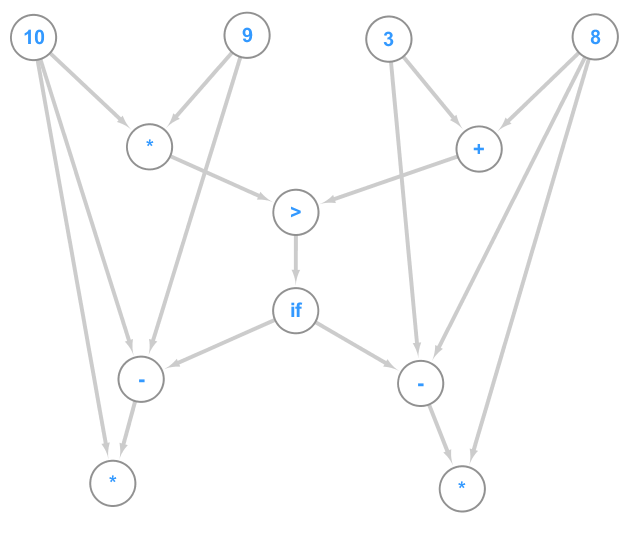
\includegraphics[scale=.7]{figuras/dataflow/pythonCodeDf.png}
    \end{minipage}
    \caption{Exemplo de conversão código para grafo de dependências.
    À esquerda pode ser visto um trecho de código em \emph{python} ao passo que à direita é exibido o grafo dataflow associado.}
    \label{fig:dataflowExemploPython}
\end{figure}

% \subsection{Sucuri} \label{sect:sucuri}

Sucuri \cite{sucuri-original} is a minimalistic Dataflow library for Python language that allows programmers to naturally exploit parallelism through dataflow execution on Von Neumann machines. Sucuri allows transparent execution on computer cluster, relying on Python mechanisms for object serialization (\emph{Pickle}).

Conceptually, a dataflow graph is comprised of nodes that represent tasks, which can be fine-grained (as instructions) or coarse-grained (as functions). Edges connecting nodes represent data-dependencies, meaning a source node will produce a result that will be used by the destination node. When a certain node receives all necessary inputs though its incident edges, it can be dispatched to execution.

Figure \ref{fig:arch} shows Sucuri's structure, where it is possible to observe three main components: \texttt{Graph}, \texttt{Scheduler} and \texttt{Worker}. 

The \texttt{Graph} is just a container object for nodes that represent a dataflow application, each containing:
\begin{itemize}
    \item The list of inputs received so far. When all necessary operands are receive a \emph{matching} occurs and node execution will be triggered.
    \item The function (computation) that should be executed when matching happens for that node.
    \item A list of destination nodes that should receive the result produced.
    \item Specific attributes, such as an unique id that can be used for assigning work to a set of nodes (like in a fork-join approach).
\end{itemize}

When used in a cluster of computers, each of the aforementioned components is replicated in each machine of the cluster, except for the Scheduler, meaning Sucuri adopts a centralized pool of tasks. In \cite{sucuri-distribuida} Sucuri authors implement and evaluate a distributed scheduler for Sucuri, but this version is not employed in this work.

\begin{figure}[htbp]
    \centering
    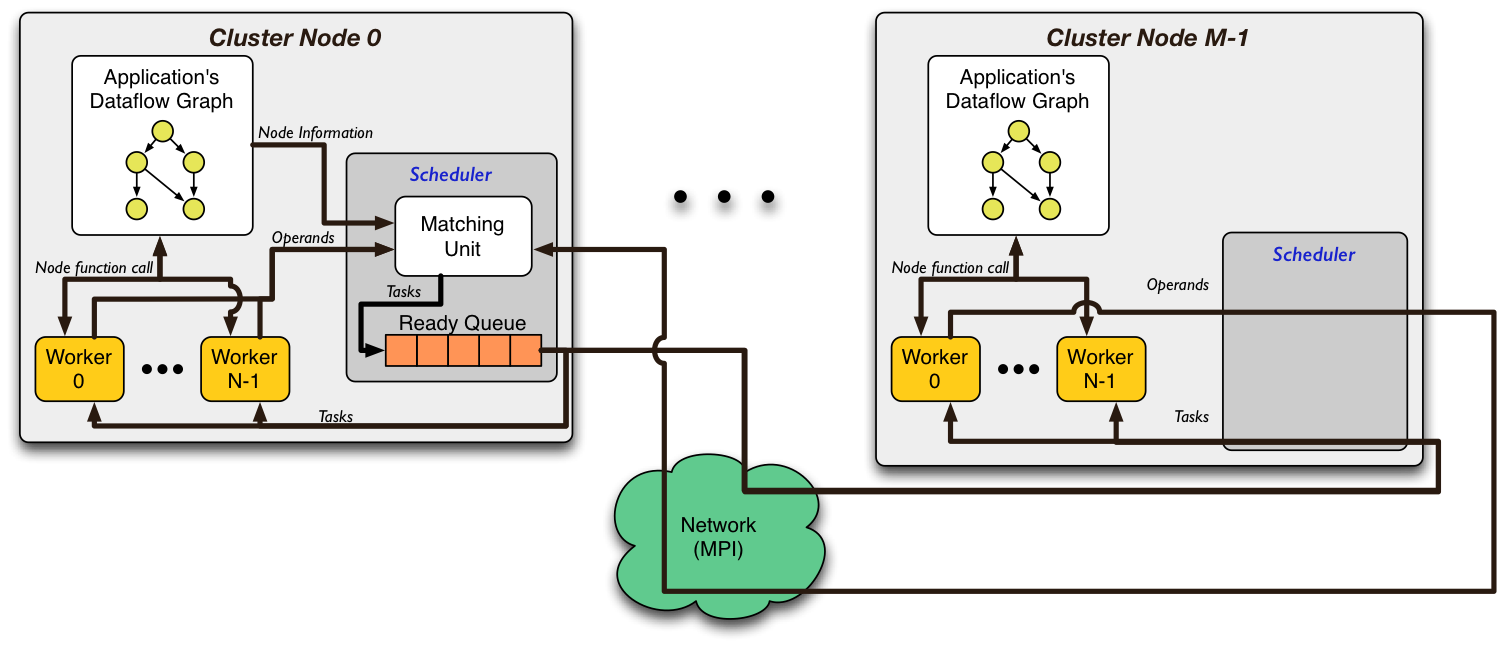
\includegraphics[scale=0.65]{figuras/dataflow/SucuriArchitectureHorizonal.png}
    \caption{The Sucuri Architecture (from \cite{sucuri-original}). The same structure is replicated in each node but only the Scheduler from Cluster Node 0 contains the Matching Unit and the Ready Queue. It is responsible for receiving operands from local Workers and from the others Schedulers and also to generate tasks and put them into the Ready Queue.}
    \label{fig:arch}
\end{figure}

The main \texttt{Scheduler}, placed at Cluster Node 0, is composed of a Matching Unit, a Ready Queue and a Waiting Queue. It is responsible for delivering all operands to the operand list of its destination Node in the Graph. If a match happens, a task is created and put in the Ready Queue. When workers are idle they will request tasks to the \texttt{Scheduler}, that would be fetched from the Ready Queue. The \texttt{Scheduler} placed in the other cluster nodes are more simple and only forwards tasks from the main \texttt{Scheduler} to their local workers and operands from their workers to the main \texttt{Scheduler}. The graph is replicated in all nodes of the Cluster but only the graph in node 0 can receive operands from the main \texttt{Scheduler}.

All communication intra-node between the main components cited above is done via shared memory and between Schedulers from different nodes is done via interface.

Each node of a Sucuri graph is associated with a function that can be implemented by programmers and pass them to node instantiation when creating the dataflow graph. After instantiating the nodes, the programmer can then proceed to connect them using the \texttt{add\_edge()} method, which basically creates a new dependency in the dataflow graph. When the scheduler dispatches a task for execution in a certain worker, that worker will call the \texttt{run()} method of the node corresponding to that task. In most cases, this \texttt{run()} method will just act as a wrapper that calls the function associated with the node during the construction of the graph and send the values returned by the function call to the main scheduler.

Sucuri also provides a set of special nodes that could help programmers devise applications that follow some parallel patterns. For example, a software pipeline application for Sucuri is presented in Fig.~\ref{fig:pipeline}. Panel $A$ shows a graph representation of this pattern and panel $B$ the Sucuri's code for this operation. Notice how new nodes are creates (lines 11-13), added to the graph (lines 17-19) and how edges connecting the nodes are defined (lines 21 and 22). Also, notice the instantiation of the scheduler (line 6) and how to start the schedule after the dataflow graph is defined (line 23).

Figure \ref{fig:pipeline} also shows how a special node \texttt{Source} receives an \emph{iterable} Python object (for instance, a list or a file descriptor) at instantiation. During program execution, the \texttt{run()} method of the \emph{Source} node will be fired only once, since this node works as a root, i.e., has no input operands from the graph and serves to initiate the computation. The execution of such method, however, will typically last until the contents of the iterable object are exhausted. By default the \texttt{Source} node will loop over the iterable object and produce several outputs (messages) that would trigger the execution of the pipeline multiple times. 

Notice that the last node of the pipeline is a special \texttt{Serializer} node, that is responsible for writing the data to a file. It is possible for the data produced by the \texttt{Source} node to be processed out of order by the second node, since the multiple tasks may be scheduled to different workers. Therefore, it is necessary to reorder the data before writing it to the file, in the \texttt{Serializer} node. For that purpose, the data produced by the \texttt{Source} node must be encapsulated in a \texttt{TaggedValue} object, which contains a \texttt{tag} attribute, indicating its position in the ordered data set. The middle node will also send the filtered data inside of a \texttt{TaggedValue} object, with the same tag of the chunk of data it received. The \texttt{Serializer} node then, upon receiving data from the filter node, will store it in a buffer sorted according to the tag. If the tag of the last piece of data received corresponds to the next data to be written to the file, the \texttt{Serializer} node proceeds to pop data from the sorted buffer and write to the file until there is a gap in the ordering, i.e. the chunk of data that is the next to be written has not arrived yet. If the data received by the \texttt{Serializer} is out of order, the node just stores it in the sorted buffer and waits for more data. The \texttt{pin\(\)} method is used to pin the node to a certain worker, which will make it only be executed by that worker. In the case of the example, we pin the nodes that performs I\/O operations on disk to the workers that have direct access to that disk. 

\begin{figure}[htbp]
    \centering
    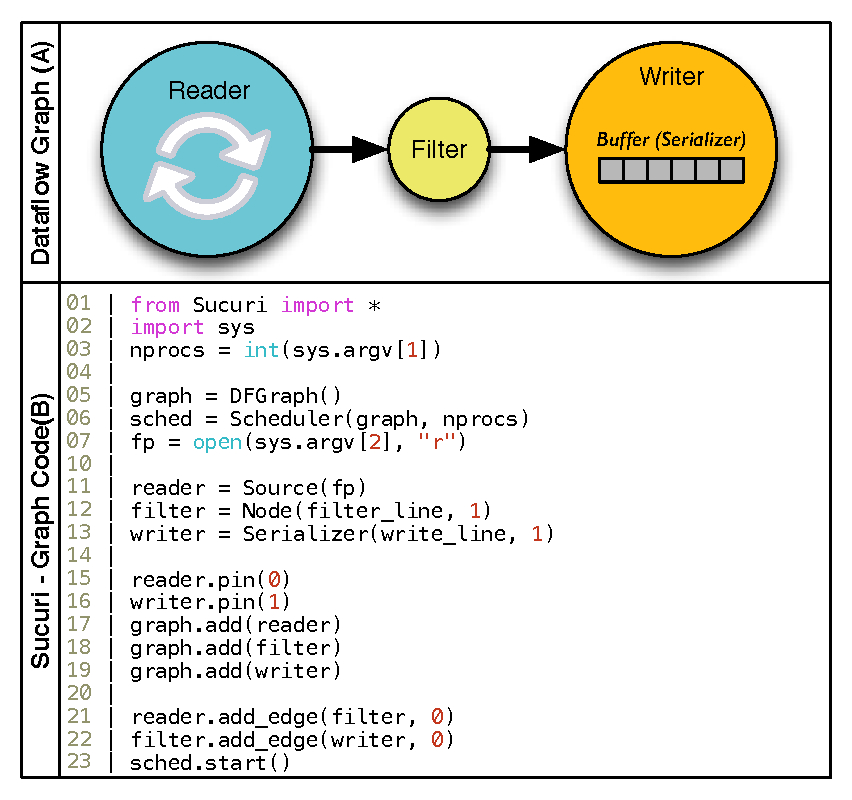
\includegraphics[scale=0.75]{figuras/dataflow/pipeline.eps} 
    \caption{Pipelining with Sucuri. 
    %The data is read from the disk by \texttt{Reader} node encapsulated in a \texttt{TaggedValue} object while a filter is applied by \texttt{Filer} node in a data read previously. As the \texttt{Filter} finish, the \texttt{Writer} node receives and store them in buffer sorted according to the tag. If the tag of the last piece of data received corresponds to the next data to be written to the file, the \texttt{Writer} node proceeds to pop data from the sorted buffer and write to the file.
    Panel $A$ shows the dataflow graph of the application, panel $B$ describes the graph using Sucuri.}
    \label{fig:pipeline}
\end{figure}

One interesting modeling feature that we explore in this paper consists in exploring coarse-grained programming in Sucuri together with fine-grained computing on GPU. This results in a heterogeneous Dataflow/Von Neumann computing, with dataflow nodes performing high performance GPU computing.
This strategy provides greater flexibility for the design of novel algorithms, with greater simplicity than adopting a single computing paradigm (dataflow or von Neumann).



\section{Dataflow} \label{sec:conceitosDataflow}
% Essa parte tá bem próxima da tese do Marzulo

Atualmente os processadores no mercado de computadores seguem, em geral, o modelo de \textit{Von Neumann}.
No referido modelo, a execução das instruções é guiada por um fluxo de controle, ou seja, segundo a ordem que aparecem no programa, desta forma se faz necessário um \textit{Program Counter} (Contador de Programa) para indicar qual a próxima instrução a ser executada.
O contador também pode ser alterado por instruções de desvio, e laços de repetição ou qualquer tipo de comando de execução condicional.

Note que este modelo é intrinsecamente sequencial. No entanto, tenta-se resgatar paralelismo em nível de instruções com técnicas como pipelining~\cite{patterson2003computerOrganization}, predição de desvio~\cite{patterson2003computerOrganization} e renomeamento de registradores~\cite{patterson2012}.

O modelo dataflow~\cite{2468, Swanson2003, 642111, Davis:1978:ASM:800094.803050, 714523, Shimada:1986:EPD:17356.17383, Kishi:1983:DDD:1067651.801661, Grafe:1989:EDP:74925.74930, 134511, Swanson:2007:WA:1233307.1233308} expõe paralelismo de forma natural.
Neste modelo, as instruções são executadas de acordo com o fluxo de dados, ou seja, assim que todos os seus operandos de entrada estiverem disponíveis.

No modelo dataflow os programas são escritos como um grafo de fluxo de dados onde os nós representam as instruções e as arestas direcionadas indicam as dependências de dados.
Assim $A \rightarrow B$ indica que $A$ produz um dado que é enviado como entrada para $B$ após ter sido processado.
Cabe lembrar que este modelo é adotado nas máquinas de Von Neumann para extrair paralelismo ao implementar o mecanismo de execução fora-de-ordem com escalonamento dinâmico baseado em fluxo de dados~\cite{tomasulo}, contudo limitado o paralelismo pela emissão das instruções que permanece seguindo o fluxo de controle.
Numa arquitetura que segue totalmente o fluxo de dados as instruções não são emitidas segundo se apresentam no programa, instruções distintas podem executar concorrentemente.

Na Figura~\ref{fig:dataflowExemploPython} pode ser visto um programa simples, à esquerda é mostrado o código e à direita sua tradução no grafo de fluxo de dados associado, note que as instruções de soma e multiplicação podem ser executadas em paralelo ou qualquer ordem sem alterar o resultado final.

\begin{figure}
    \centering
    \begin{minipage}{.3\textwidth}
        \centering
\begin{minted}{python}
a = 10
b = 9
c = 3
d = 8
e = a * b
f = c + d
if e > f:
  g = (a - b) * a
else:
  g = (c - d) * d
\end{minted}
    \end{minipage}
    \begin{minipage}{.675\textwidth}
        \centering %width=.655\linewidth
        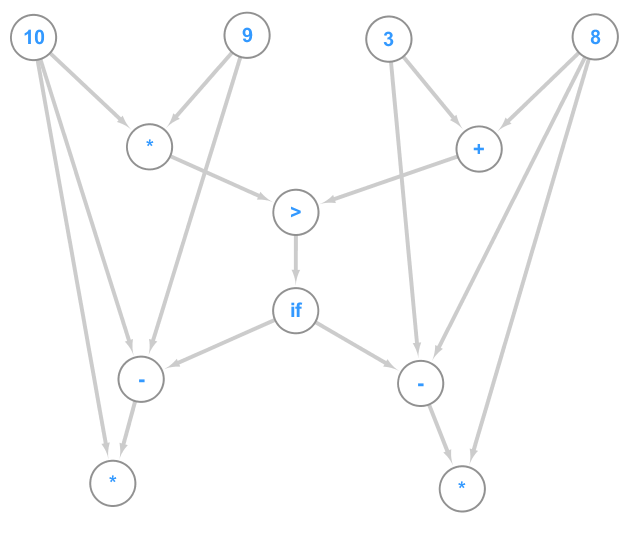
\includegraphics[scale=.7]{figuras/dataflow/pythonCodeDf.png}
    \end{minipage}
    \caption{Exemplo de conversão código para grafo de dependências.
    À esquerda pode ser visto um trecho de código em \emph{python} ao passo que à direita é exibido o grafo dataflow associado.}
    \label{fig:dataflowExemploPython}
\end{figure}

% \subsection{Sucuri} \label{sect:sucuri}

Sucuri \cite{sucuri-original} is a minimalistic Dataflow library for Python language that allows programmers to naturally exploit parallelism through dataflow execution on Von Neumann machines. Sucuri allows transparent execution on computer cluster, relying on Python mechanisms for object serialization (\emph{Pickle}).

Conceptually, a dataflow graph is comprised of nodes that represent tasks, which can be fine-grained (as instructions) or coarse-grained (as functions). Edges connecting nodes represent data-dependencies, meaning a source node will produce a result that will be used by the destination node. When a certain node receives all necessary inputs though its incident edges, it can be dispatched to execution.

Figure \ref{fig:arch} shows Sucuri's structure, where it is possible to observe three main components: \texttt{Graph}, \texttt{Scheduler} and \texttt{Worker}. 

The \texttt{Graph} is just a container object for nodes that represent a dataflow application, each containing:
\begin{itemize}
    \item The list of inputs received so far. When all necessary operands are receive a \emph{matching} occurs and node execution will be triggered.
    \item The function (computation) that should be executed when matching happens for that node.
    \item A list of destination nodes that should receive the result produced.
    \item Specific attributes, such as an unique id that can be used for assigning work to a set of nodes (like in a fork-join approach).
\end{itemize}

When used in a cluster of computers, each of the aforementioned components is replicated in each machine of the cluster, except for the Scheduler, meaning Sucuri adopts a centralized pool of tasks. In \cite{sucuri-distribuida} Sucuri authors implement and evaluate a distributed scheduler for Sucuri, but this version is not employed in this work.

\begin{figure}[htbp]
    \centering
    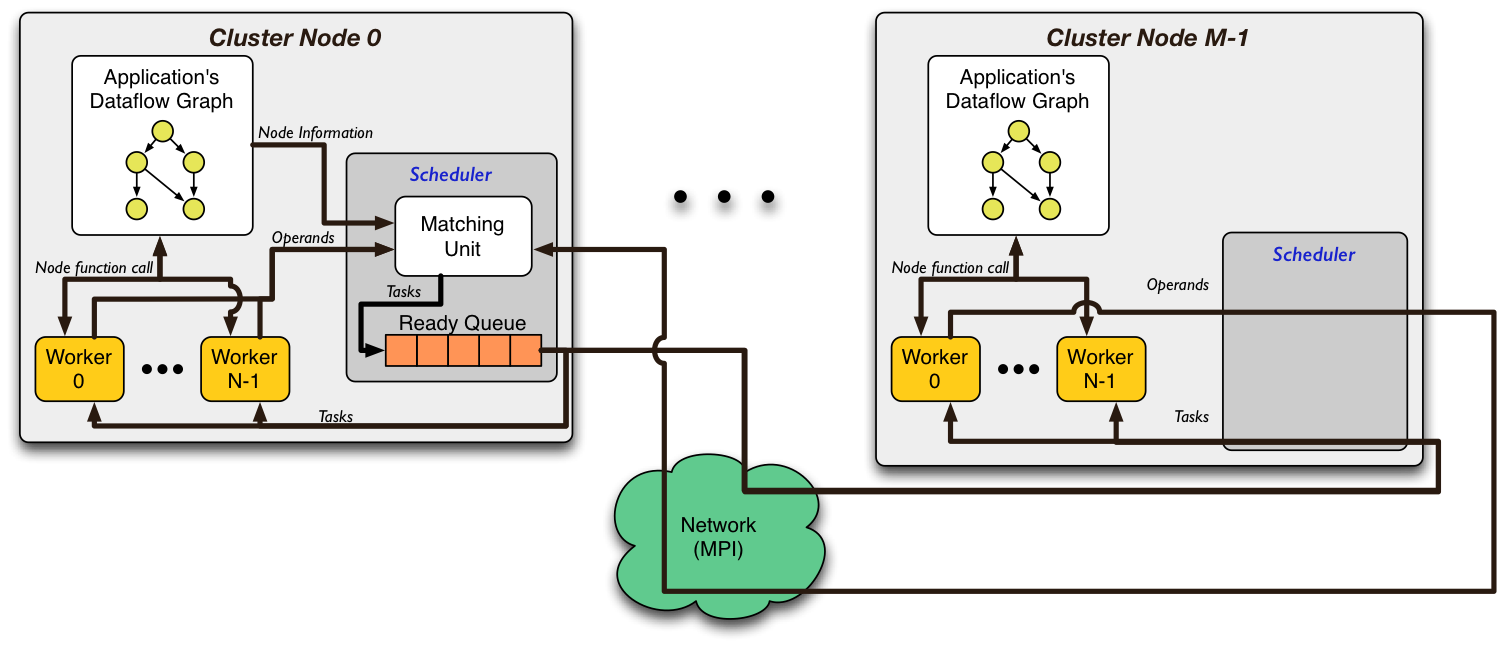
\includegraphics[scale=0.65]{figuras/dataflow/SucuriArchitectureHorizonal.png}
    \caption{The Sucuri Architecture (from \cite{sucuri-original}). The same structure is replicated in each node but only the Scheduler from Cluster Node 0 contains the Matching Unit and the Ready Queue. It is responsible for receiving operands from local Workers and from the others Schedulers and also to generate tasks and put them into the Ready Queue.}
    \label{fig:arch}
\end{figure}

The main \texttt{Scheduler}, placed at Cluster Node 0, is composed of a Matching Unit, a Ready Queue and a Waiting Queue. It is responsible for delivering all operands to the operand list of its destination Node in the Graph. If a match happens, a task is created and put in the Ready Queue. When workers are idle they will request tasks to the \texttt{Scheduler}, that would be fetched from the Ready Queue. The \texttt{Scheduler} placed in the other cluster nodes are more simple and only forwards tasks from the main \texttt{Scheduler} to their local workers and operands from their workers to the main \texttt{Scheduler}. The graph is replicated in all nodes of the Cluster but only the graph in node 0 can receive operands from the main \texttt{Scheduler}.

All communication intra-node between the main components cited above is done via shared memory and between Schedulers from different nodes is done via interface.

Each node of a Sucuri graph is associated with a function that can be implemented by programmers and pass them to node instantiation when creating the dataflow graph. After instantiating the nodes, the programmer can then proceed to connect them using the \texttt{add\_edge()} method, which basically creates a new dependency in the dataflow graph. When the scheduler dispatches a task for execution in a certain worker, that worker will call the \texttt{run()} method of the node corresponding to that task. In most cases, this \texttt{run()} method will just act as a wrapper that calls the function associated with the node during the construction of the graph and send the values returned by the function call to the main scheduler.

Sucuri also provides a set of special nodes that could help programmers devise applications that follow some parallel patterns. For example, a software pipeline application for Sucuri is presented in Fig.~\ref{fig:pipeline}. Panel $A$ shows a graph representation of this pattern and panel $B$ the Sucuri's code for this operation. Notice how new nodes are creates (lines 11-13), added to the graph (lines 17-19) and how edges connecting the nodes are defined (lines 21 and 22). Also, notice the instantiation of the scheduler (line 6) and how to start the schedule after the dataflow graph is defined (line 23).

Figure \ref{fig:pipeline} also shows how a special node \texttt{Source} receives an \emph{iterable} Python object (for instance, a list or a file descriptor) at instantiation. During program execution, the \texttt{run()} method of the \emph{Source} node will be fired only once, since this node works as a root, i.e., has no input operands from the graph and serves to initiate the computation. The execution of such method, however, will typically last until the contents of the iterable object are exhausted. By default the \texttt{Source} node will loop over the iterable object and produce several outputs (messages) that would trigger the execution of the pipeline multiple times. 

Notice that the last node of the pipeline is a special \texttt{Serializer} node, that is responsible for writing the data to a file. It is possible for the data produced by the \texttt{Source} node to be processed out of order by the second node, since the multiple tasks may be scheduled to different workers. Therefore, it is necessary to reorder the data before writing it to the file, in the \texttt{Serializer} node. For that purpose, the data produced by the \texttt{Source} node must be encapsulated in a \texttt{TaggedValue} object, which contains a \texttt{tag} attribute, indicating its position in the ordered data set. The middle node will also send the filtered data inside of a \texttt{TaggedValue} object, with the same tag of the chunk of data it received. The \texttt{Serializer} node then, upon receiving data from the filter node, will store it in a buffer sorted according to the tag. If the tag of the last piece of data received corresponds to the next data to be written to the file, the \texttt{Serializer} node proceeds to pop data from the sorted buffer and write to the file until there is a gap in the ordering, i.e. the chunk of data that is the next to be written has not arrived yet. If the data received by the \texttt{Serializer} is out of order, the node just stores it in the sorted buffer and waits for more data. The \texttt{pin\(\)} method is used to pin the node to a certain worker, which will make it only be executed by that worker. In the case of the example, we pin the nodes that performs I\/O operations on disk to the workers that have direct access to that disk. 

\begin{figure}[htbp]
    \centering
    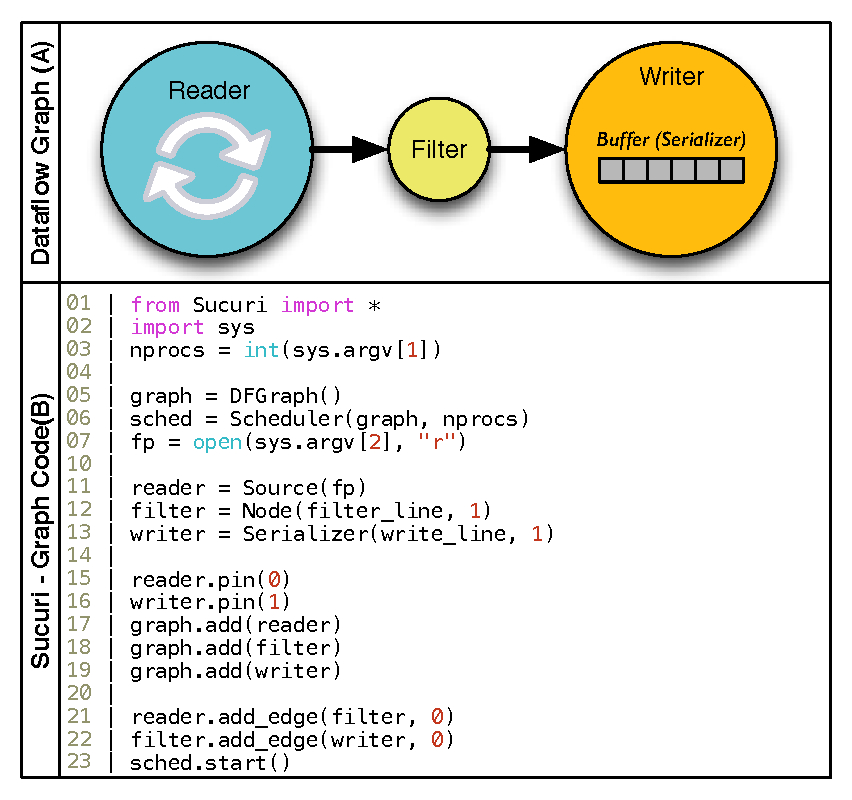
\includegraphics[scale=0.75]{figuras/dataflow/pipeline.eps} 
    \caption{Pipelining with Sucuri. 
    %The data is read from the disk by \texttt{Reader} node encapsulated in a \texttt{TaggedValue} object while a filter is applied by \texttt{Filer} node in a data read previously. As the \texttt{Filter} finish, the \texttt{Writer} node receives and store them in buffer sorted according to the tag. If the tag of the last piece of data received corresponds to the next data to be written to the file, the \texttt{Writer} node proceeds to pop data from the sorted buffer and write to the file.
    Panel $A$ shows the dataflow graph of the application, panel $B$ describes the graph using Sucuri.}
    \label{fig:pipeline}
\end{figure}

One interesting modeling feature that we explore in this paper consists in exploring coarse-grained programming in Sucuri together with fine-grained computing on GPU. This results in a heterogeneous Dataflow/Von Neumann computing, with dataflow nodes performing high performance GPU computing.
This strategy provides greater flexibility for the design of novel algorithms, with greater simplicity than adopting a single computing paradigm (dataflow or von Neumann).


